\chapter{Results}

% Eine mögliche Struktur der Arbeit sieht wie folgt aus:

% \begin{enumerate}
%     \item \textbf{Einleitung}\\
%         In der \emph{kurzen} Einleitung wird die Motivation für die Arbeit
%         dargestellt und ein Einblick in die kommenden Kapitel gegeben.
%     \item \textbf{Theoretische Grundlagen}\\
%         Alles was an theoretischen Grundlagen benötigt wird, sollte auch eher kurz gehalten werden.
%         Statt Grundlagenwissen zu präsentieren, eher auf die entsprechenden Lehrbücher verweisen.
%         Etwa: Tiefer gehende Informationen zur klassischen Mechanik entnehmen Sie bitte \cite{kuypers}.
%     \item \textbf{Ergebnisse} \\
%         Der eigentliche Teil der Arbeit, das was getan wurde.
%     \item \textbf{Zusammenfassung und Ausblick} \\
%         Zusammenfassung der Ergebnisse, Optimierungsmöglichkeiten, mögliche weitergehende Untersuchungen.
% \end{enumerate}

% Die Gliederung sollte auf der einen Seite nicht zu fein sein, auf der anderen Seite
% sollten sich klar unterscheidende Abschnitte auch kenntlich gemacht werden.

% In der hier verwendeten \KOMAScript-Klasse \texttt{scrbook} ist die oberste Gliederungsebene,
% die in der Bachelorarbeit verwendet werden sollte, das \texttt{\textbackslash chapter}.

% Ein Kapitel sollte erst dann in tiefere Gliederungsebenen unterteilt werden, wenn es auch wirklich etwas zu unterteilen gibt. 
% Es sollte keine Kapitel mit nur einem Unterkapitel (\texttt{\textbackslash section}) geben.

% In dieser Vorlage ist die Tiefe des Inhaltsverzeichnisses auf \texttt{chapter} und \texttt{section} beschränkt. 
% Möchten Sie diese Beschränkung aufheben, entfernen Sie den Befehl
% \begin{verbatim}
%             \setcounter{tocdepth}{1}
% \end{verbatim}
% aus der Präambel oder ändern Sie den Zahlenwert entsprechend. Das Inhaltsverzeichnis sollte für eine Bachelorarbeit auf eine Seite passen.

The analysis will be split into two parts, with the first part focussing on the probabilities and frequencies of coincident events, while the second part 
focusses on understanding the physical nature of what constitutes a coincident event. 

\section{Probabilities of coincident events}%\label{sec:muon_coincidence}

As explained in \ref{sec:coin} the probability function of coincidence events against total events can be estimated to follow a poisson distribution.
A theoretical distribution for different trigger windows is shown in figure~\ref{fig:coin_rate_rate}. 

\begin{figure}
    \centering
    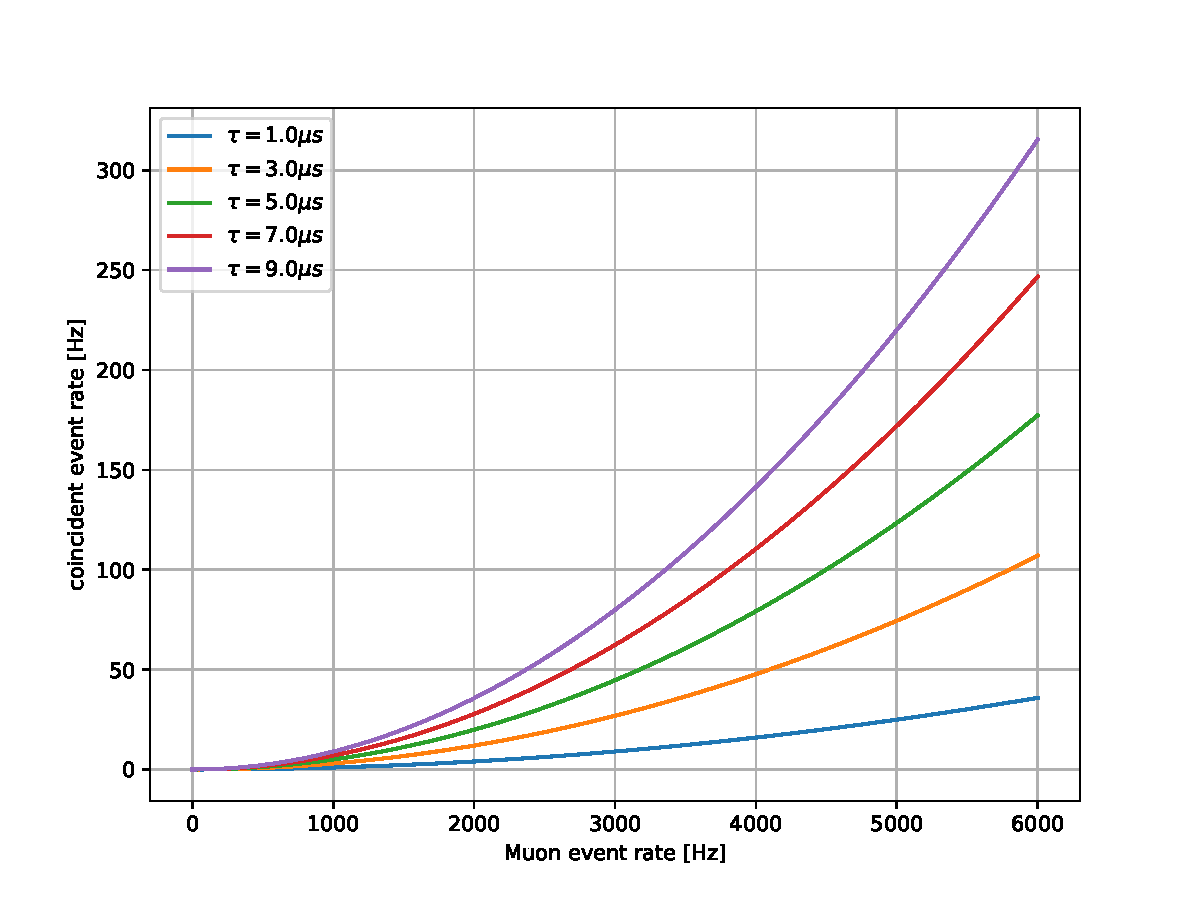
\includegraphics[width=0.7\textwidth]{Plots/coincidence_rate_poisson.pdf}
    \caption{A graph showing the relation between the muon event rate and the corresponding event rate assuming a poisson distributed muon event rate.}
    \label{fig:coin_rate_rate}
\end{figure}

In order to put this into a meaningful context, a relation of the muon event rate and their corresponding energy is extracted from a monte carlo simulation.
With this data describing a step function $rate(energy)$, equation~\ref{eq:multi_rate} can be used to visualize the relation between the muon energy and their 
corresponding rate of coincident events. Equivalent calculations are made on a zenith angle spectrum, for which the data is extracted from the same set of monte 
carlo data. Both of these distributions, along with the corresponding intervals, in which the coincidence probability exceeds \SI{0.1}{\percent}, are shown in 
figure~\ref{fig:coin_rate_combined}.

\begin{figure}[ht]
    \centering
    \begin{subfigure}[b]{\textwidth}
        \centering
        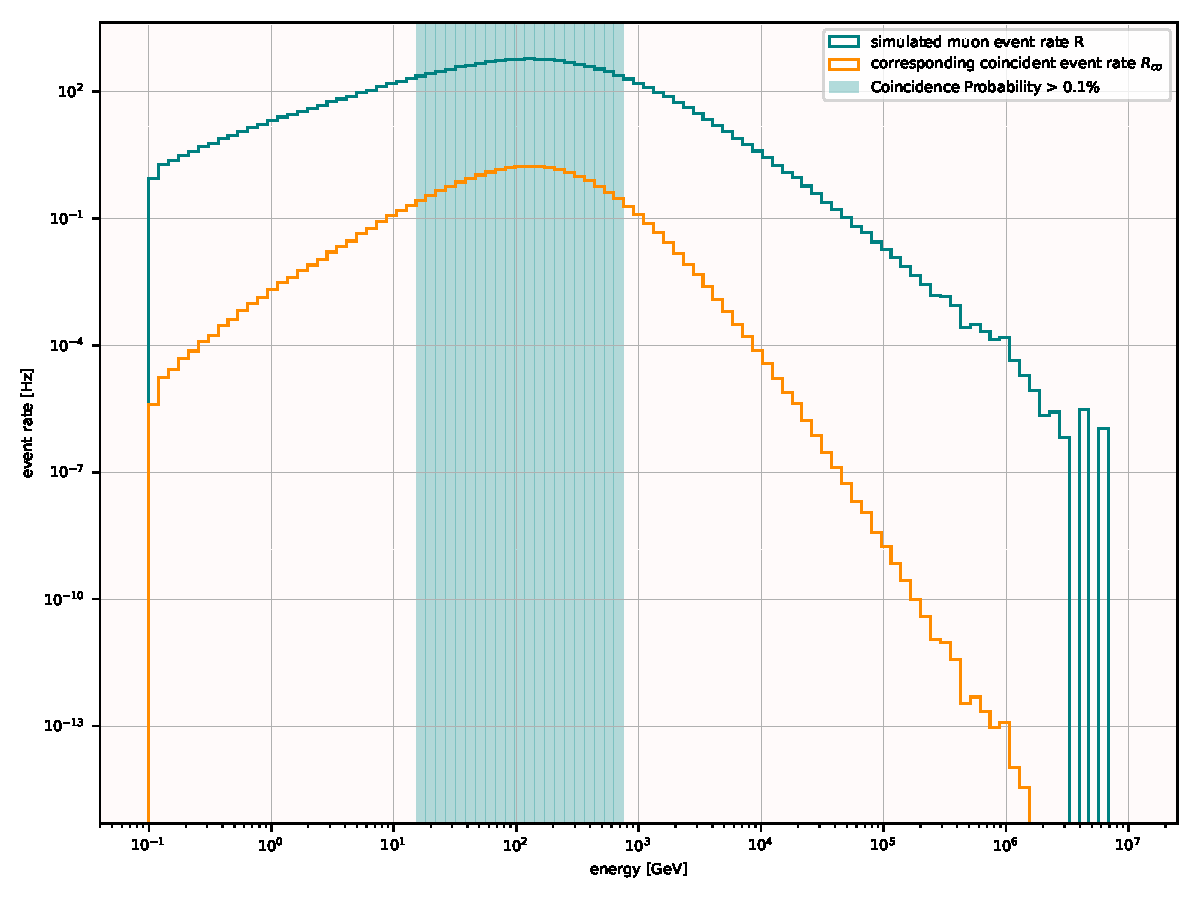
\includegraphics[width=0.7\textwidth]{Plots/coincidence_rate_energy.pdf}
    \end{subfigure}
    \vspace{1em} % Optional vertical space between the plots
    \begin{subfigure}[b]{\textwidth}
        \centering
        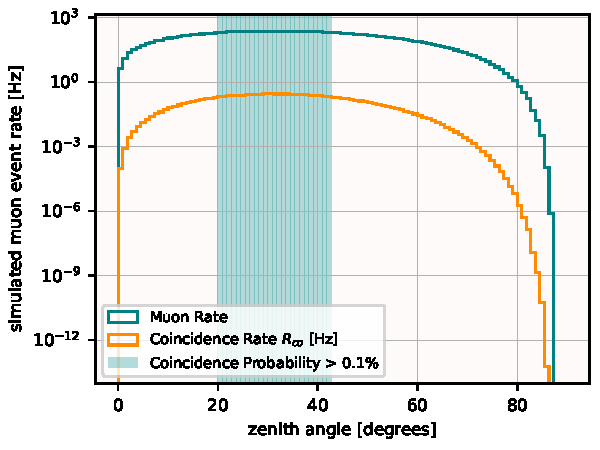
\includegraphics[width=0.7\textwidth]{Plots/coincidence_rate_zenith.pdf}
    \end{subfigure}
    \caption{Comparisons of the muon event rate and corresponding coincident event rate on energy and zenith angle spectra.}
    \label{fig:coin_rate_combined}
\end{figure}


Both histograms only show the theoretical coincidence event rate for a fixed trigger window $\tau$. However, diffrent triggers have diffrent readout windows, which 
can significantly change the probability of a coincident event. Treating the readout window as a variable, the coincident event probabilities can be visualized in 
a heat map to get a look at the effects of differing readout windows, as shown in figure~\ref{fig:heatmaps_combined}.

\begin{figure}[ht]
    \centering
    \begin{subfigure}[b]{\textwidth}
        \centering
        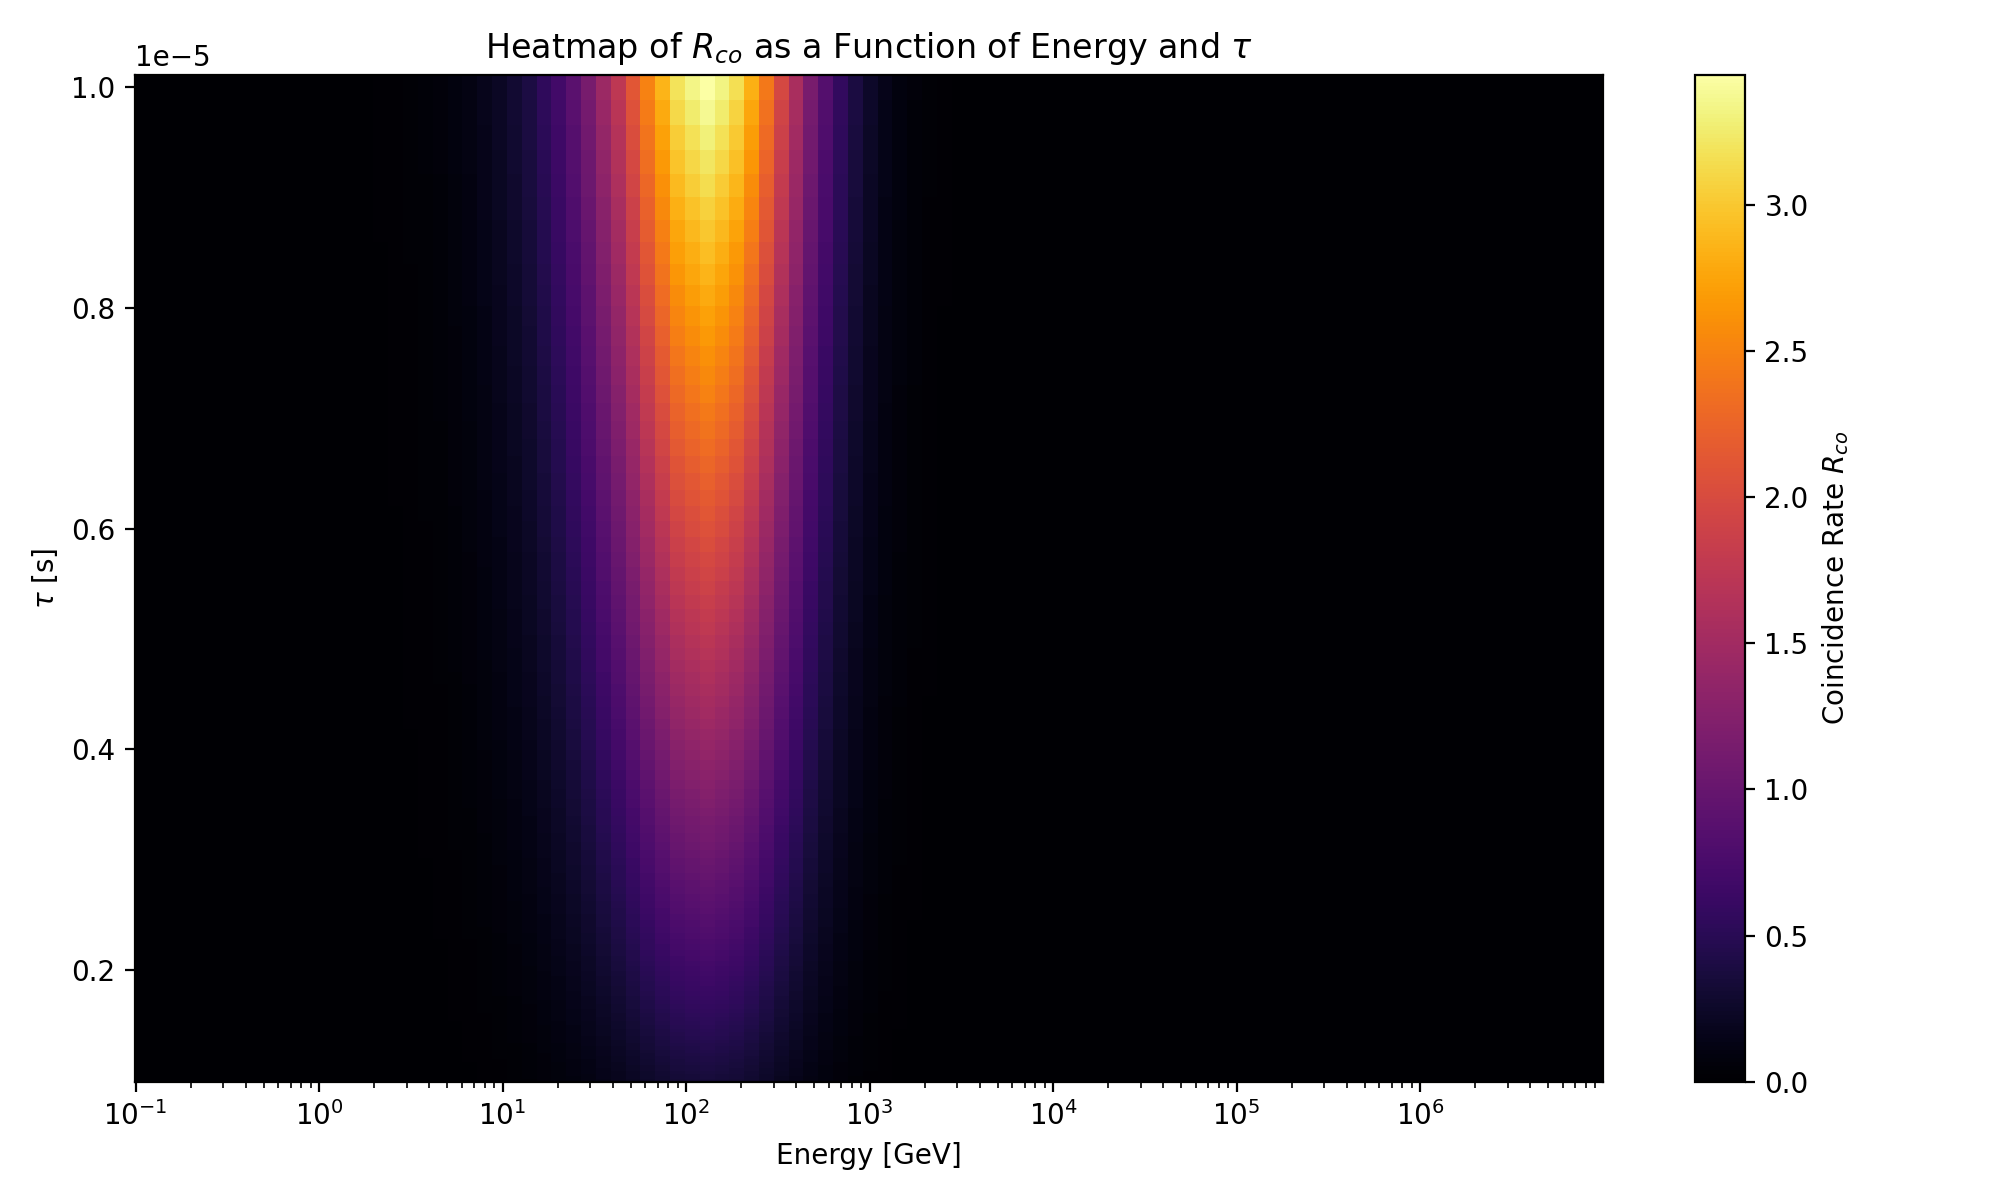
\includegraphics[width=0.7\textwidth]{Plots/heatmap_energy.png}
    \end{subfigure}
    \vspace{1em} % Optional vertical space between the plots
    \begin{subfigure}[b]{\textwidth}
        \centering
        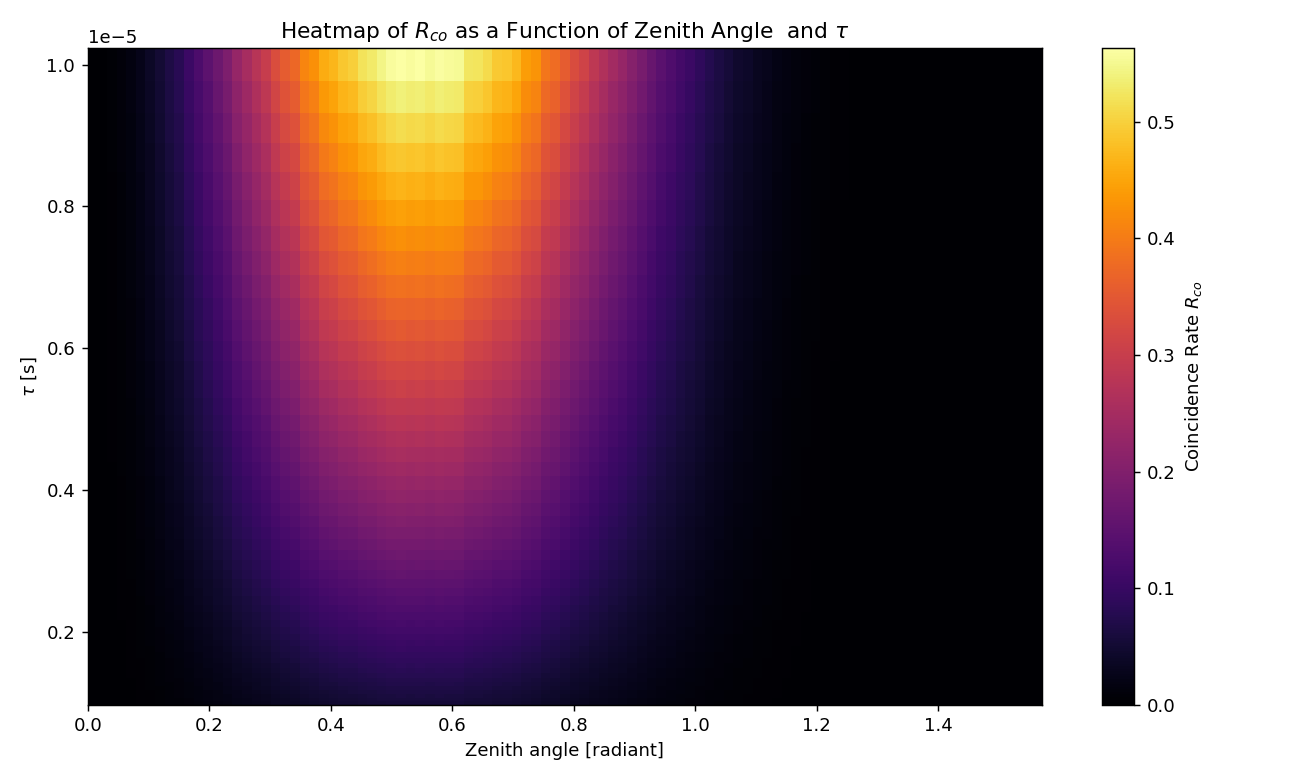
\includegraphics[width=0.7\textwidth]{Plots/heatmap_zenith.png}
    \end{subfigure}
    \caption{Prototypes of the heatmaps for energy and zenith angle spectra.}
    \label{fig:heatmaps_combined}
\end{figure}



\section{Analysis of the Fixed Rate Trigger}

The functionality of the FRT is described in section~\ref{sec:daq}. In the following section, the spectrum of the data aquired by the FRT will be analyzed in 
detail. For the analysis of the FRT, an event will mean everyting that is measured within a single trigger window. 

The following Plots give an overview of the charge distribution of the signals collected by the FRT. Firstly, the charge distribution making up a 
single event is shown in the Histograms~\ref{fig:single_charge_hist}. One entry consist of one signal hitting one DOM measuring a charge.
As expected, the counts follow a visible poisson distribution on the charge spectrum. 

\begin{figure}
    \centering
    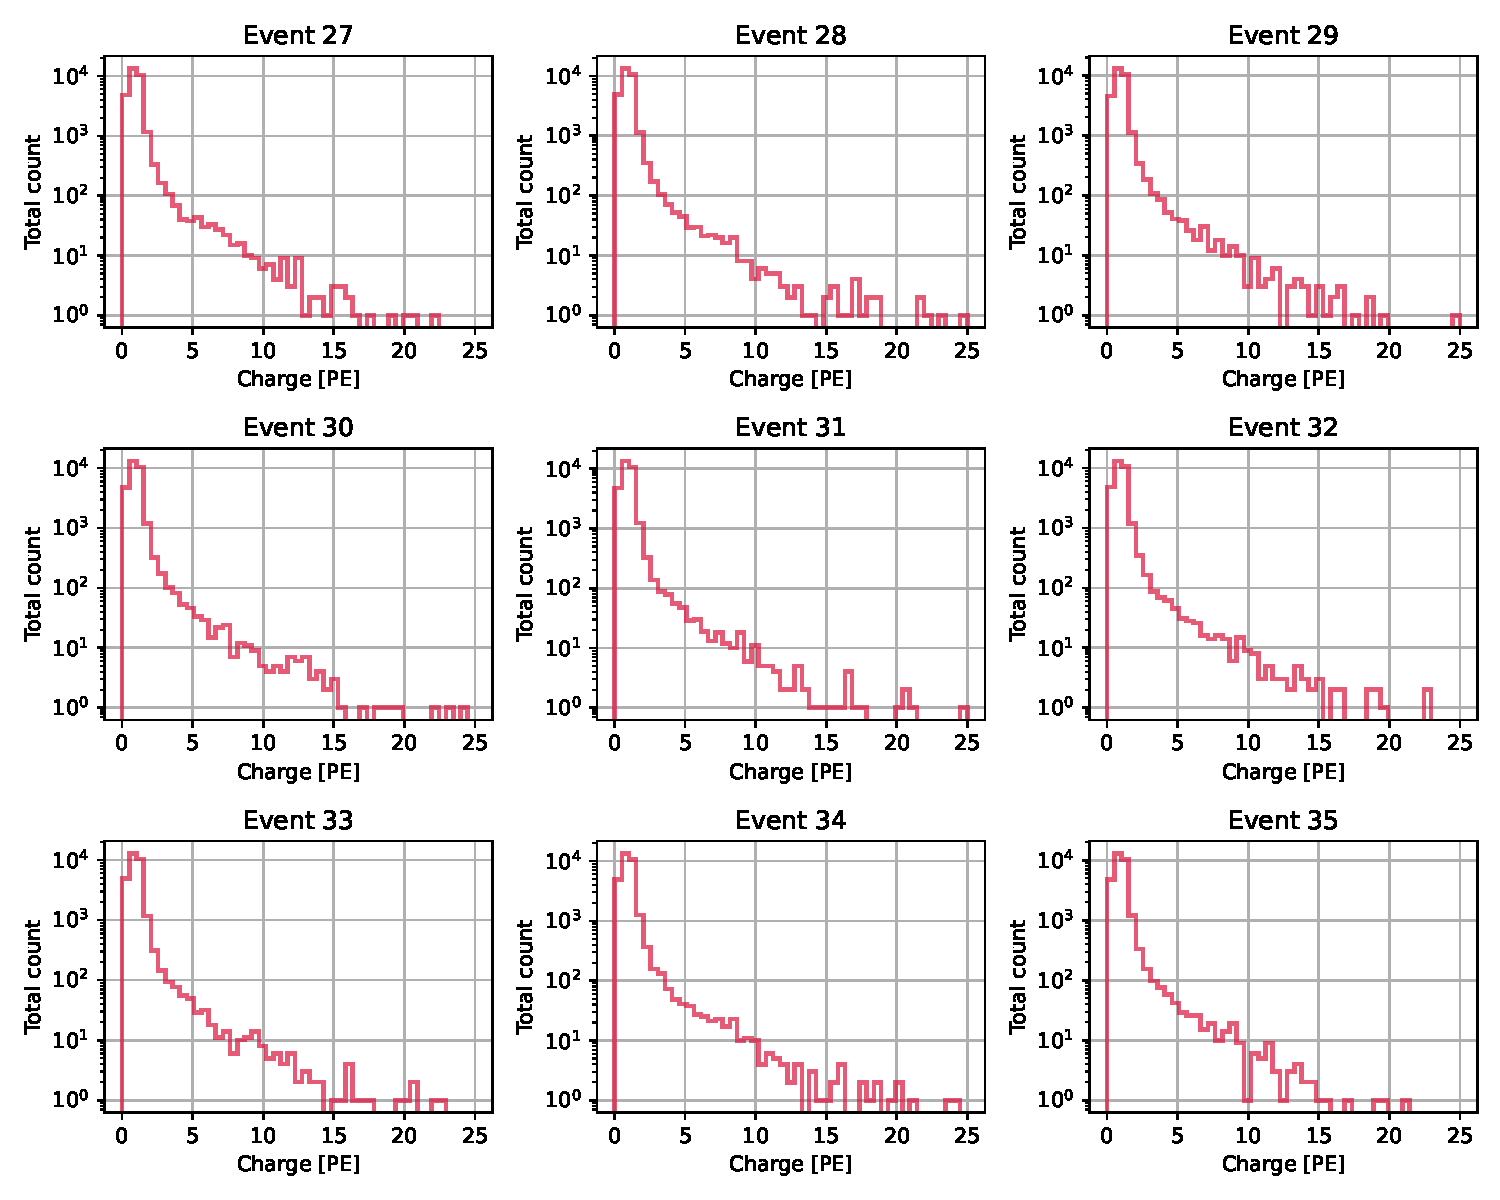
\includegraphics[width=0.7\textwidth]{Plots/single_charge_hist.pdf}
    \caption{histograms of the charge distribution of a subset of FRT events from April 2016.}
    \label{fig:single_charge_hist}
\end{figure}

In the histograms~\ref{fig:monthly_charge_hist} the data is grouped together in a way that shows one entry as one event where the charges are summed up, meaning the 
integrals of the histograms~\ref{fig:single_charge_hist} would each make up one event. 

\begin{figure}
    \centering
    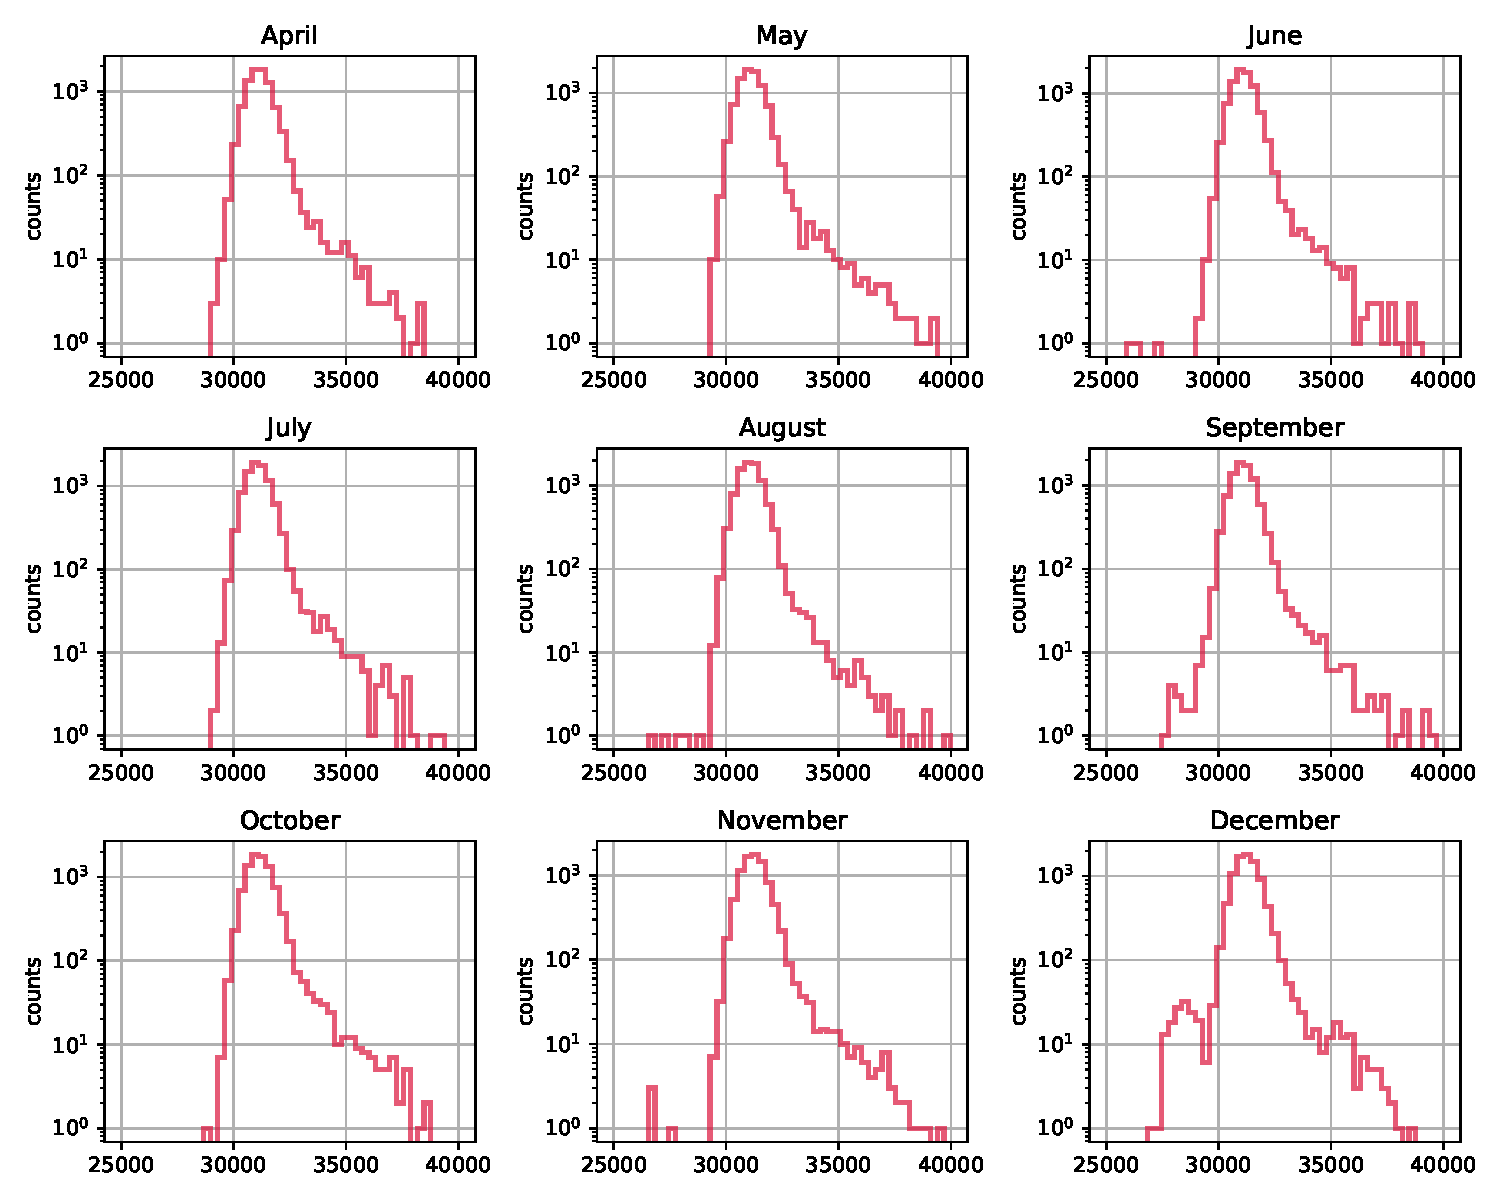
\includegraphics[width=0.7\textwidth]{Plots/monthly_charge_hist.pdf}
    \caption{histograms of the charge distribution of all events making up entire months of 2016.}
    \label{fig:monthly_charge_hist}
\end{figure}

Best visible in the histogram for May, up to a charge value of around \SI{33000}{PE} the count rate follows a pretty clear normal distribution, which is followed 
by an exponential decline. If the background noise, whatever it might be, follows a normal distribution, a sensible idea would be to fit a gauss for the charge 
values up to the critical point, after which the distribution type changes. This would allow a look into the spectrum of ''pure'' noise in IceCube, aswell as provide 
some insight on the spectrum of significant signals. (Dieser ganze Teil ergibt irgendwie doch keinen sinn oder ? soll ich die plots trotzdem drin lassen und 
beschreiben? oder lieber ganz raus lassen, wenn keine weitere analyse damit gemacht wird? ich habe auch nicht mehr im kopf, woran es nochmal lag, dass die charges
da so groß drin waren)
In order to verify the sensibilitly of this appraoch, a deeper look is taken into the data collected by the FRT. The approach is to compare the data of 
Q-Frames with the corresponding data of P-frames for the same time period of one entire month. As explained in detail in section~\ref{sec:daq}, the Q-Frame 
saves the entire readout window as one event, while the P-frames only save data making up significant physical processes. A comparison of the total counts on a 
spectrum of charge deposited in the detector is visualized in figure~\ref{fig:frt_mu_sub_comp}. 

\begin{figure}
    \centering
    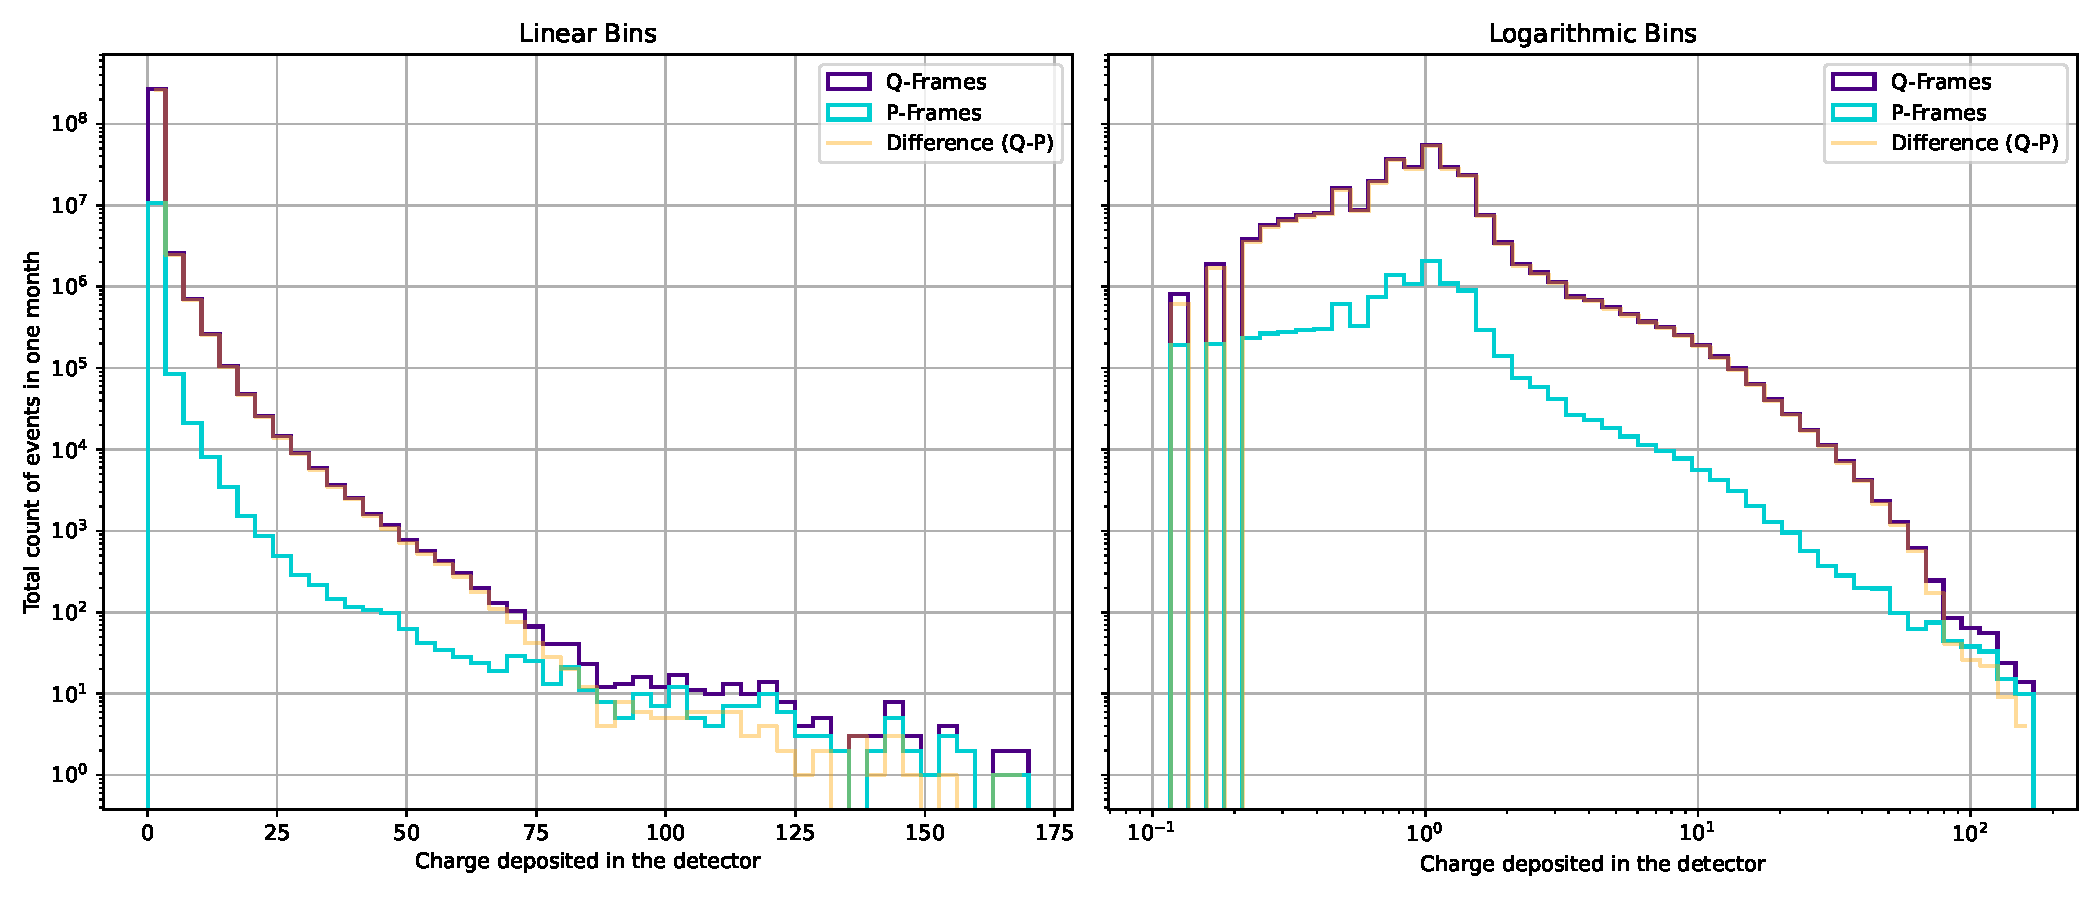
\includegraphics[width=0.7\textwidth]{Plots/q_p_comp.pdf}
    \caption{A comparison between the counts of Q-Frame and P-Frame Signals.}
    \label{fig:frt_mu_sub_comp}
\end{figure}


Comparing the two distributions, the most noticible aspect is how similar they look, to the point where they are almost identical in their structure up to a 
certain charge. The total counts vary significantly, which is to be expected considering that the data of the Q-Frames accompasses everything being measured during the 
trigger window, unlike the P-frame data. Also visible is the tendency for the P-frame data to make up a much higher percentile of the total counts of the Q-frame data.
This is also within 
expectation, since signals with higher energy usually stem from relevant physical process which are saved in P-frames. Even though the counts at the very largest 
charge values are dominated by the P-frames, it is rather unexpected to see this close of a similarity in the distributions at the charge spectrum between
\num{0} and \num{50}~\unit{PE}, where the vast majority of signals fall into. The expectation would be for the P-frame events to have an average charge significantly
larger than that of the Q-frame events. This does not appear to be the case judging by this data. Another interesting aspect of the P-frame data's distribution can be 
seen in the right subplot of figure~\ref{fig:frt_mu_sub_comp}. There are \num{386094} counts making up about \SI{3.61}{\percent} of the total P-frame counts within 
a charge interval below \num{0.25}~\unit{PE}. This is very suspicious considering that the PMTs are not capable of detecting any signal under this threshold,
see~\cite{einstein}. This might be some kind of bug in the processing of the data. For the Q-frames, the same behavior is visible. However, a bug like this 
existing for the data that should already be filtered might lead to the assumption that other 'insignificant' data exists inside of the P-frames. 

% explain it

Within these P-frames, where all of the physically significant processes are occuring, we can further filter out specific events. Not all P-frames are created by 
passing the same kind of condition. In fact, there are \num{31} unique filters sorting out different types of physical events. (sind die filter eigentlich wirklich 
das, wodurch die p frames erstellt werden ? wenn nicht, wie sonst ? )
For an overview on how different events are classified by these filters, some of them are displayed in comparison to the whole P-Frame data in 
figure~\ref{fig:filtermask}. 

\begin{figure}
    \centering
    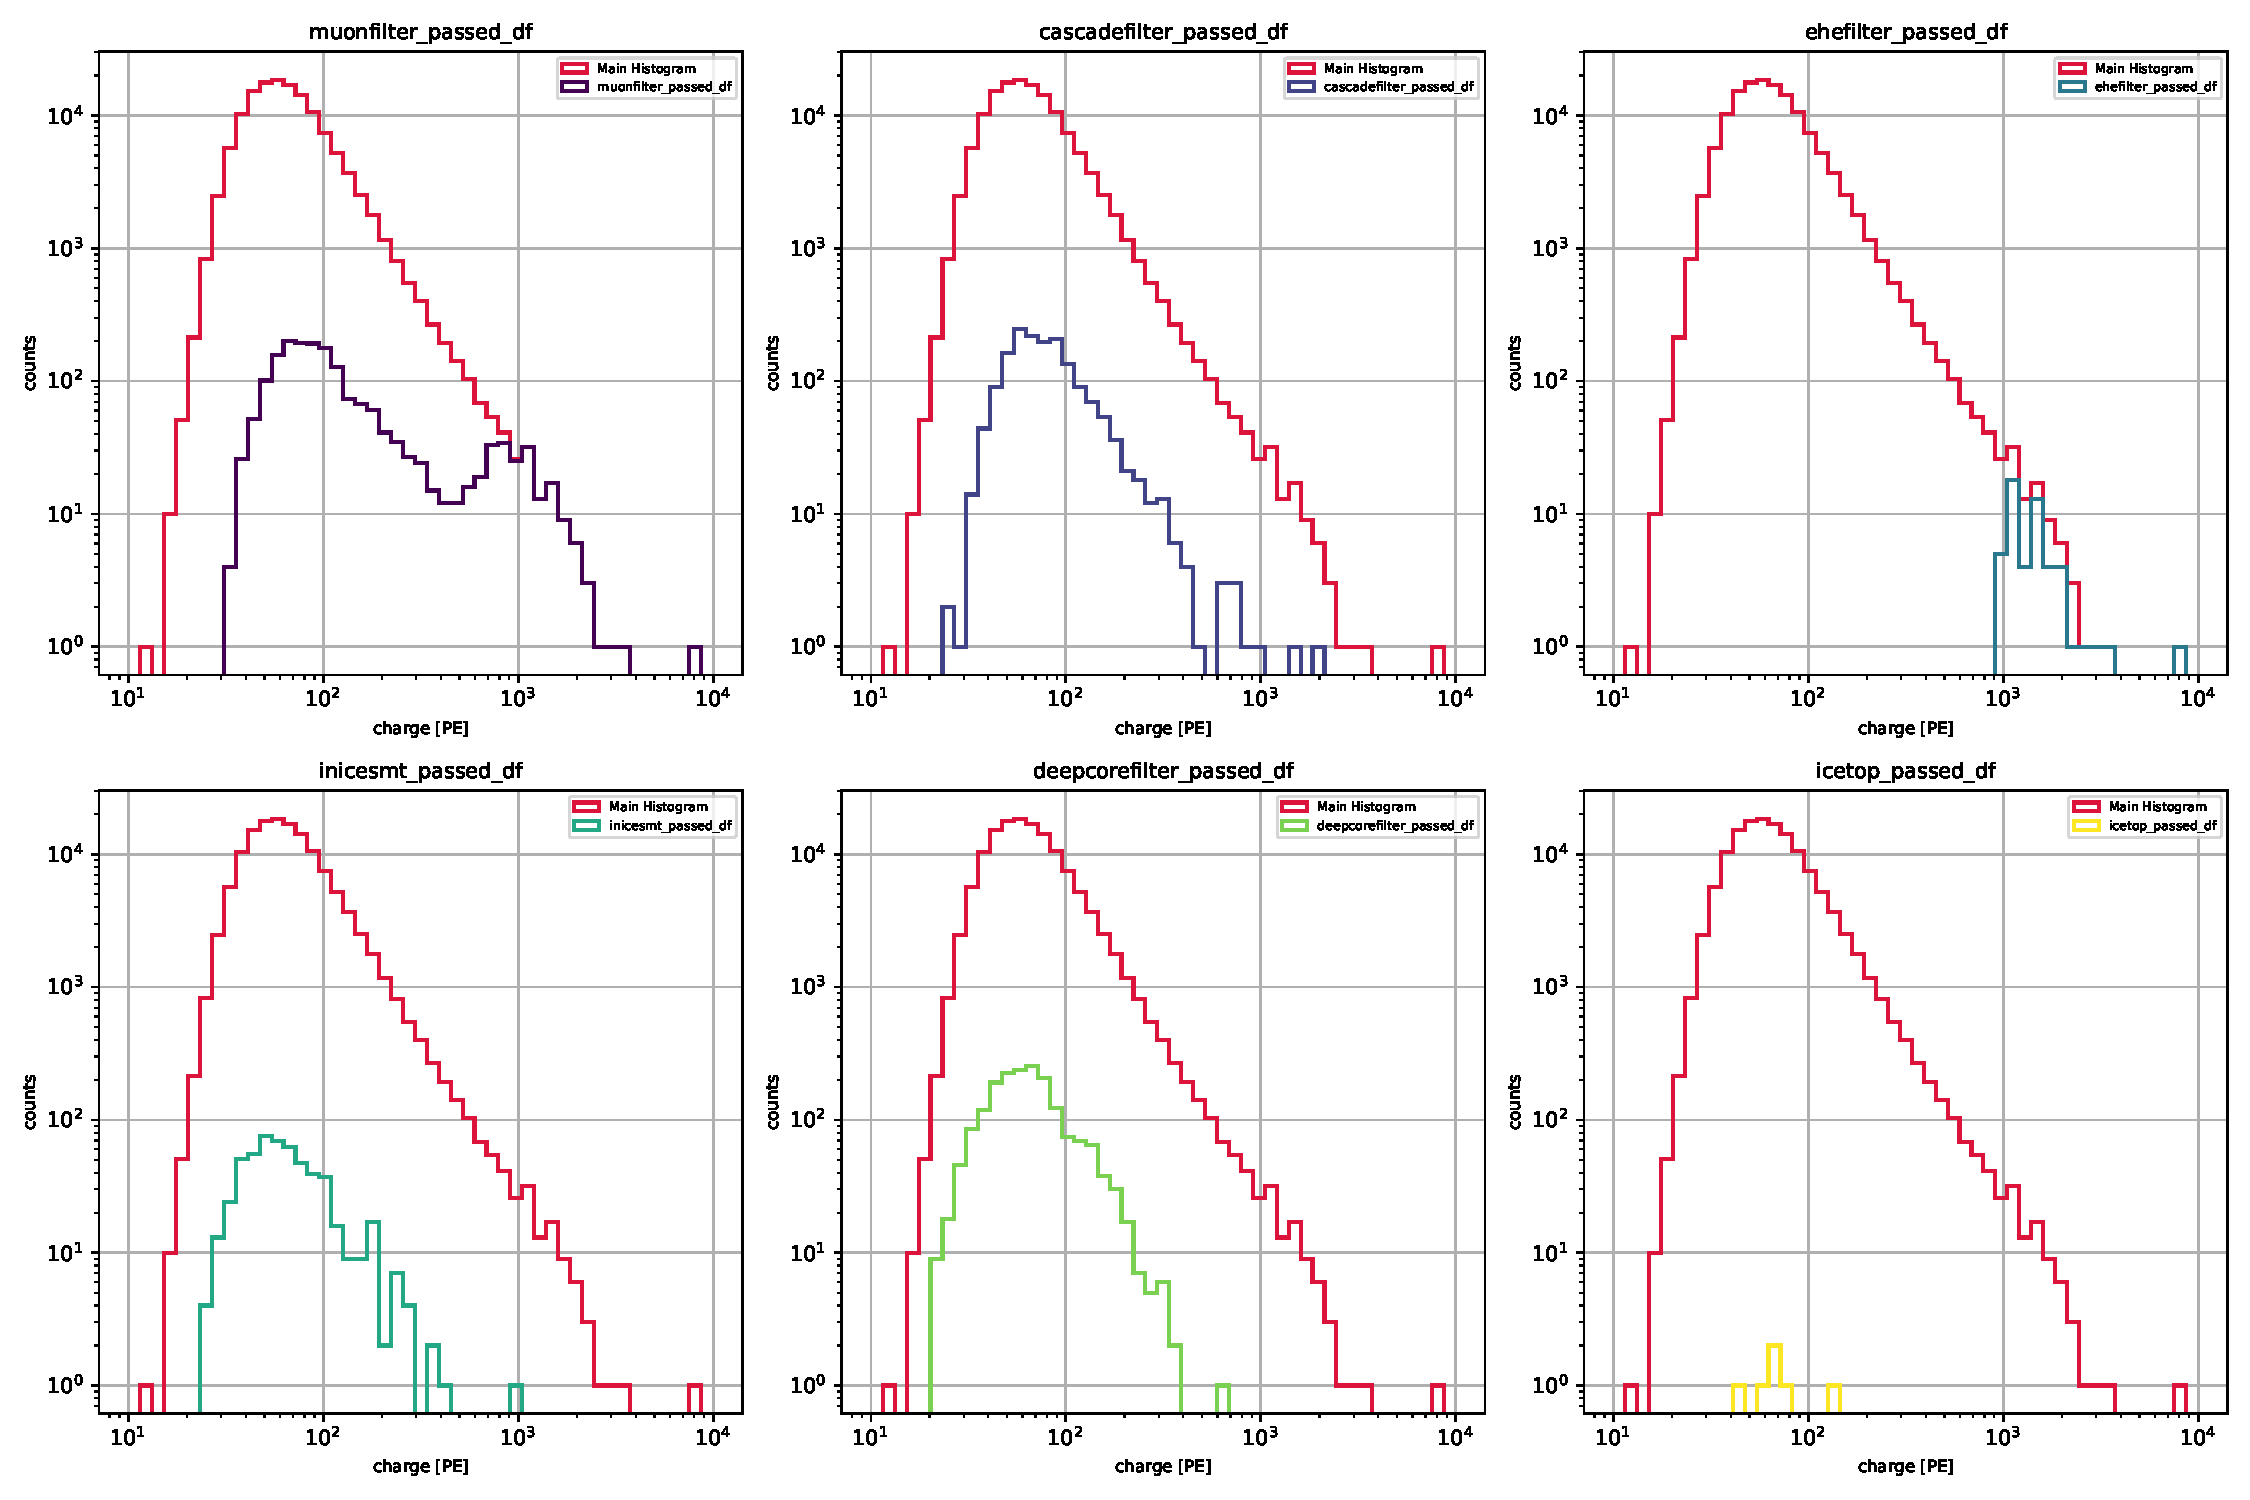
\includegraphics[width=0.7\textwidth]{Plots/selected_filters_subplot.pdf}
    \caption{A Distribution of Signals passing various Filters.}
    \label{fig:filtermask}
\end{figure}

The most significant of these histograms is the one showing the distribution of subevents passing the muon filter. 
Similarly to the comparison in~\ref{fig:frt_mu_sub_comp}, for the majority of subevents, the distributions match each other quite well in terms of their shape, up 
to a around \num{400}~\unit{PE}, where the subevents passing the muon filter start to make up a larger portion of all events. For any subevent measuring a charge of 
at least \num{1000}~\unit{PE}, the muon filter is passed.  

Another noticible aspect is the relatively low percentile of total subevents passing the muon filter. As discussed in ~\cite{einstein}, muon events are supposed to make 
up the vast majority of physical events in IceCube. However, the muon subevents determined by its filter only make up \SI{1}{\percent} of the total counts. 
This might be explainable if the comparison was made between muon subevents and Q-frame subevents, but comparing them to the subevents that should only consist of  
physically relevant events, the expectation would be for the muons to make up the vast majority of these subevents, passing the muon filter. This might be another clue 
that the P-frames created in the FRT data, could still have some sort of noise in them. 

Regardless of why the data shows the mentioned trends, the unavoidable conlusion is that it is not possible to distinguish noise from signal in a trivial way, based 
on this data. This forces the following analysis in a different direction, than originally planned. The subsequent part of the thesis will thus focus on a detailled 
analysis of data collected by FRT, in order to reevaluate its use for the study of coincident events. 




\section{for chat gpt}

In order to dive deeper into the characteristics of the FRT events, the signals measured by the detector are analyzed, focussing individual 
DOMs. For this, the mean and the standard deviation of the charges for each DOM is calculated over a period of time of \num{47}, in order to check for any anomalies
within individual DOMs. Figure~47 shows the distribution of the mean charges of every single DOM in the detector. As visible in the heatmap, the mean charges seem to 
be quite evenly distributed throughout the DOMs, with the exeption of the DOM (61,13), which shows an unusually high mean charge of \num{5.08}~\unit(PE). Another 
notable aspect, although not easily visible, is the slightly higher mean charge around the 35th OM, which will be examined at a later point. Some of bins, representing 
the individual DOMs, are completely empty, which 
might point to a defect. 


\begin{figure}
    \centering
    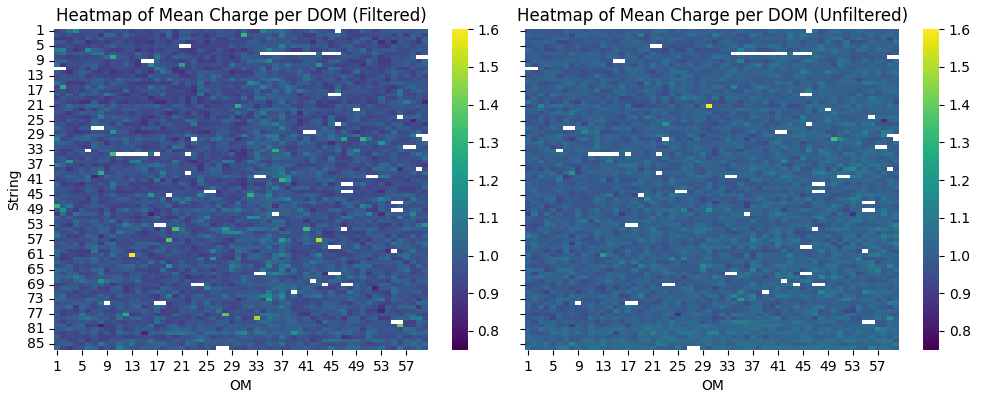
\includegraphics[width=0.7\textwidth]{Plots/mean_charge_all_dom.png}
    \caption{heatmap of p-frames and q-frames mean charges.}
\end{figure}

Another heat map in figure~47 shows the distribution of mean charges and their standard deviations of the DOMs. This is shown for the Q-frames and P-frames 
respectively. Expectedly, the P-frames contain more signals with a higher mean charge aswell as larger standard variation. However, aligning with previous observations
in figures~\ref{fig:frt_mu_sub_comp} and~\ref{fig:filtermask}, the vast majority of signals are of the same magnitude in mean charge and variance as the signals in the 
Q-frames.

\begin{figure}
    \centering
    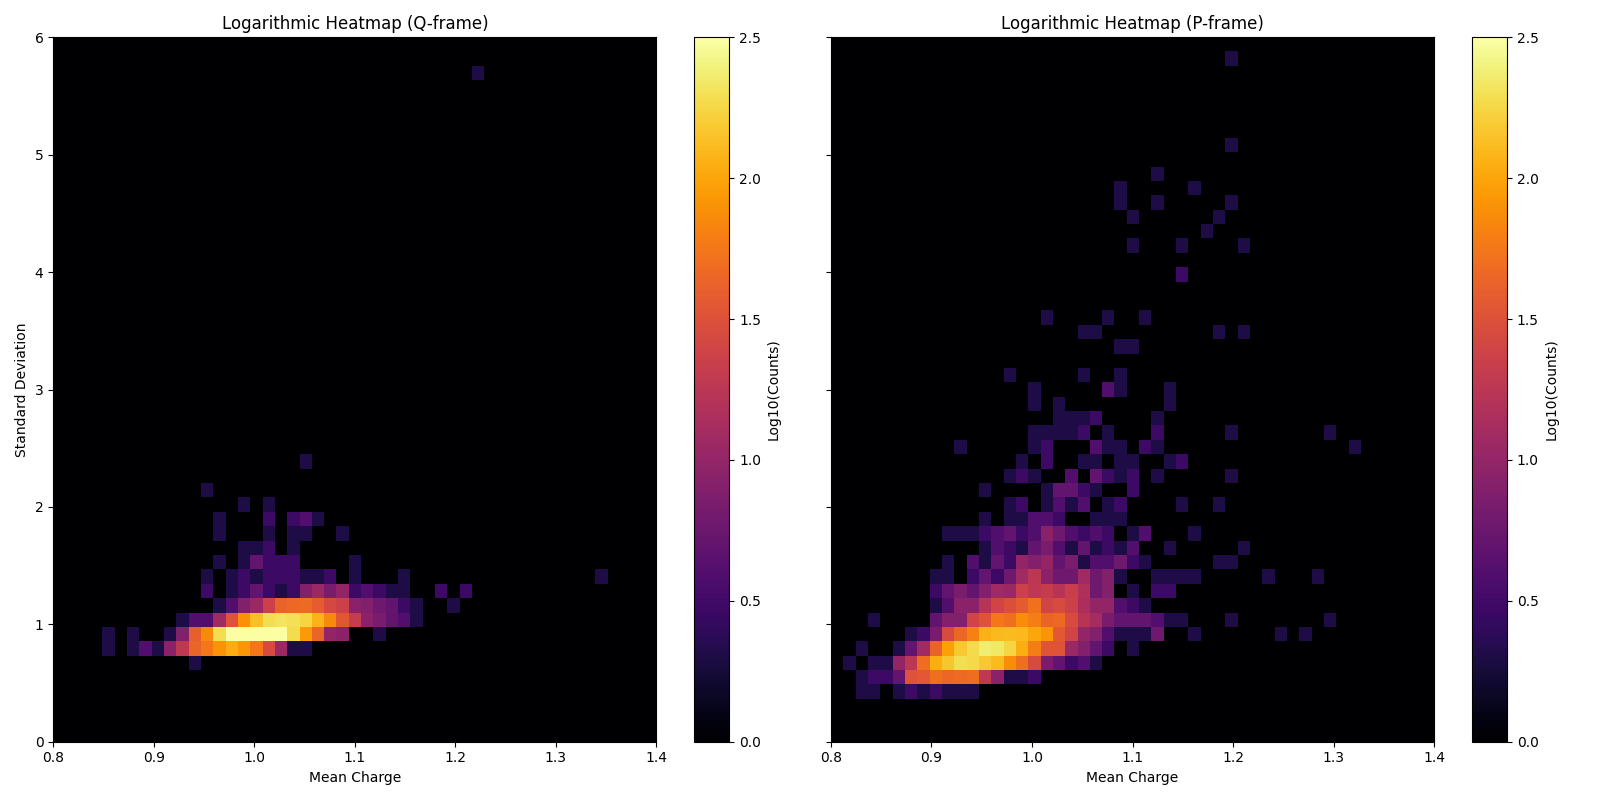
\includegraphics[width=0.7\textwidth]{Plots/mean_std_charge.png}
    \caption{mean charges distribution comparison p- and q-frames}
\end{figure}

Layering the charge per time distributions of the individual DOMs, clear peaks of charges are visible. This is done for the P-frames for all the signals above a 
certain mean charge and std threshold. Here are the plots visualizing this:

\begin{figure}
    \centering
    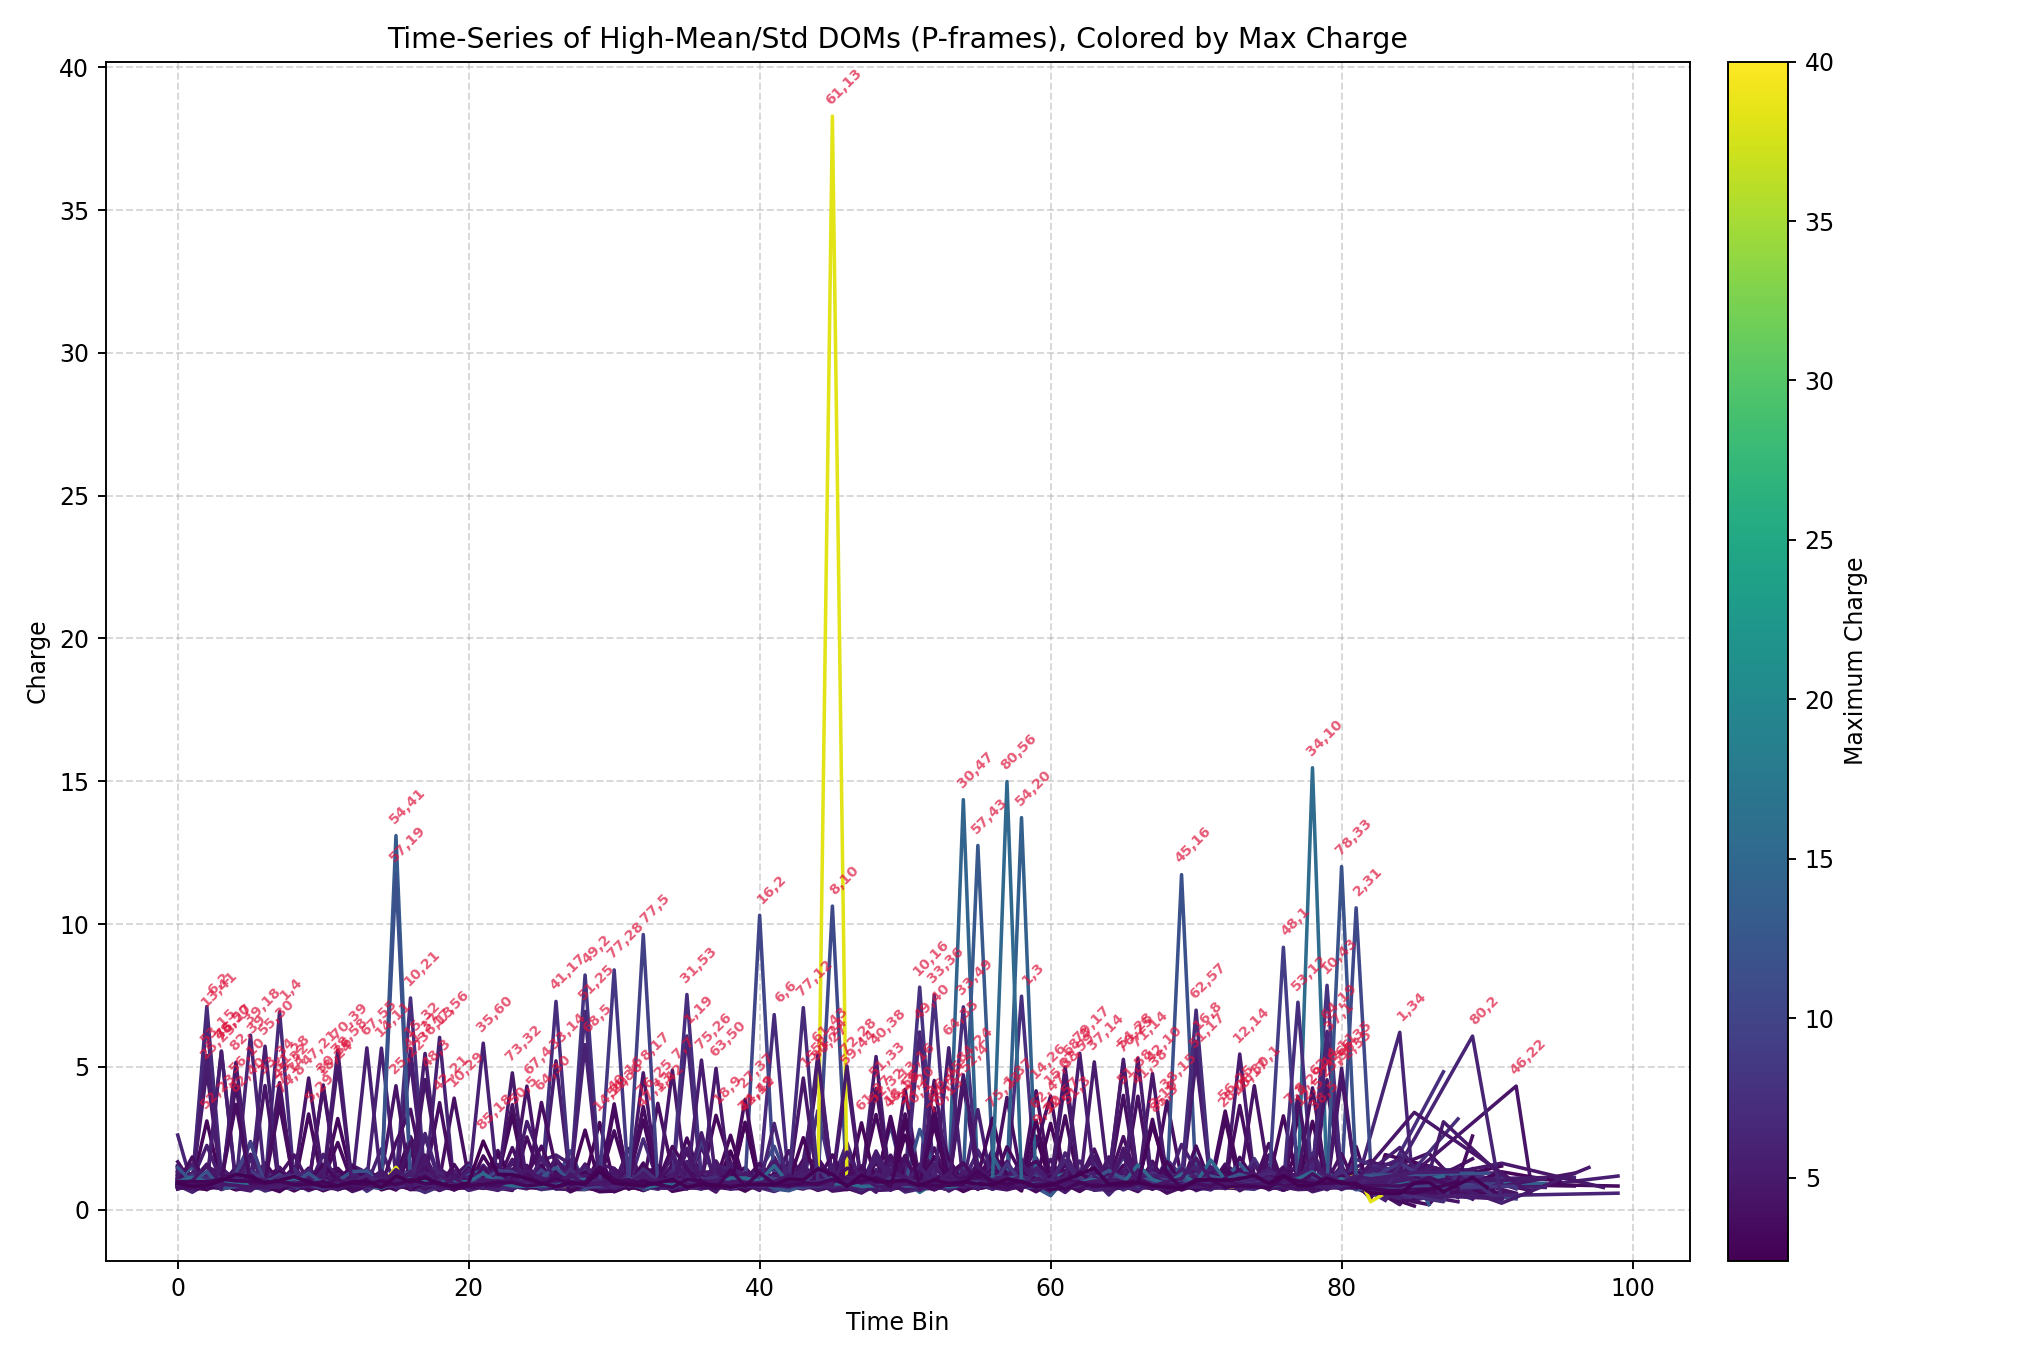
\includegraphics[width=0.7\textwidth]{Plots/p_high_mean_charges_t.png}
    \caption{p high mean charges}
\end{figure}
\begin{figure}
    \centering
    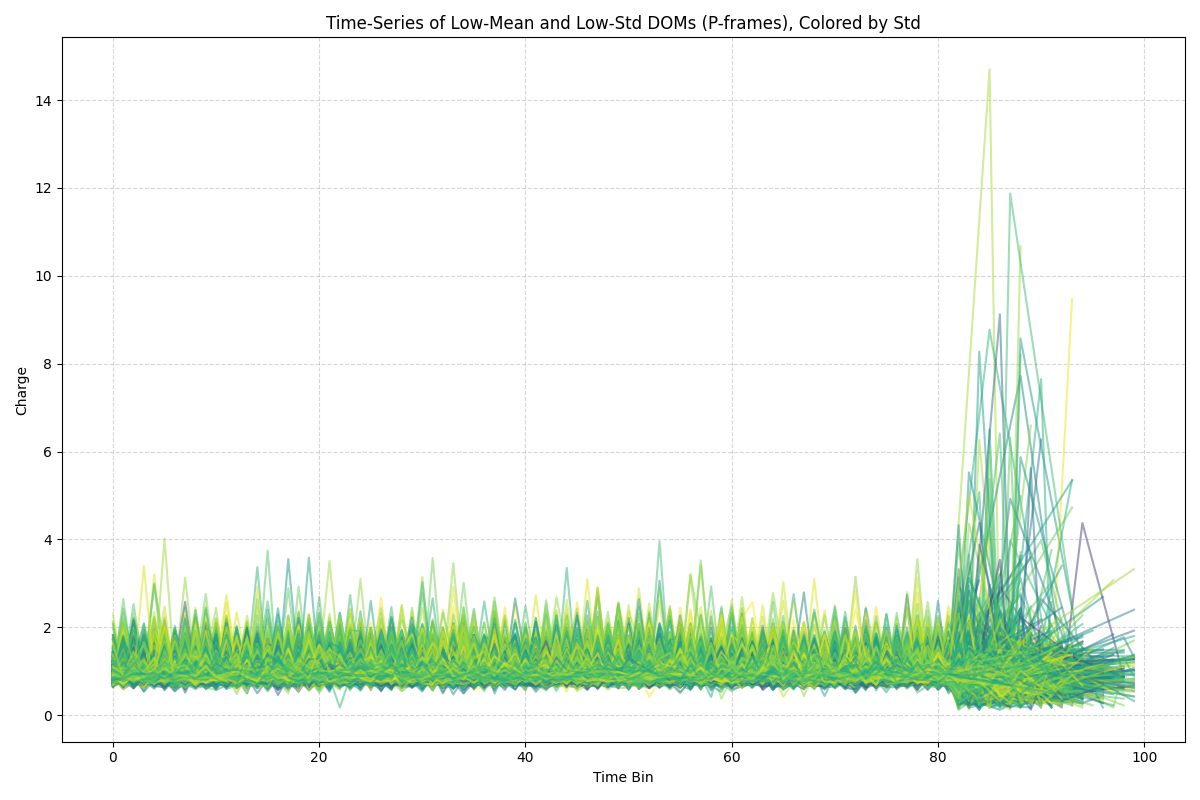
\includegraphics[width=0.7\textwidth]{Plots/q_high_mean_charges_t.png}
    \caption{p low mean charges}
\end{figure}
\begin{figure}
    \centering
    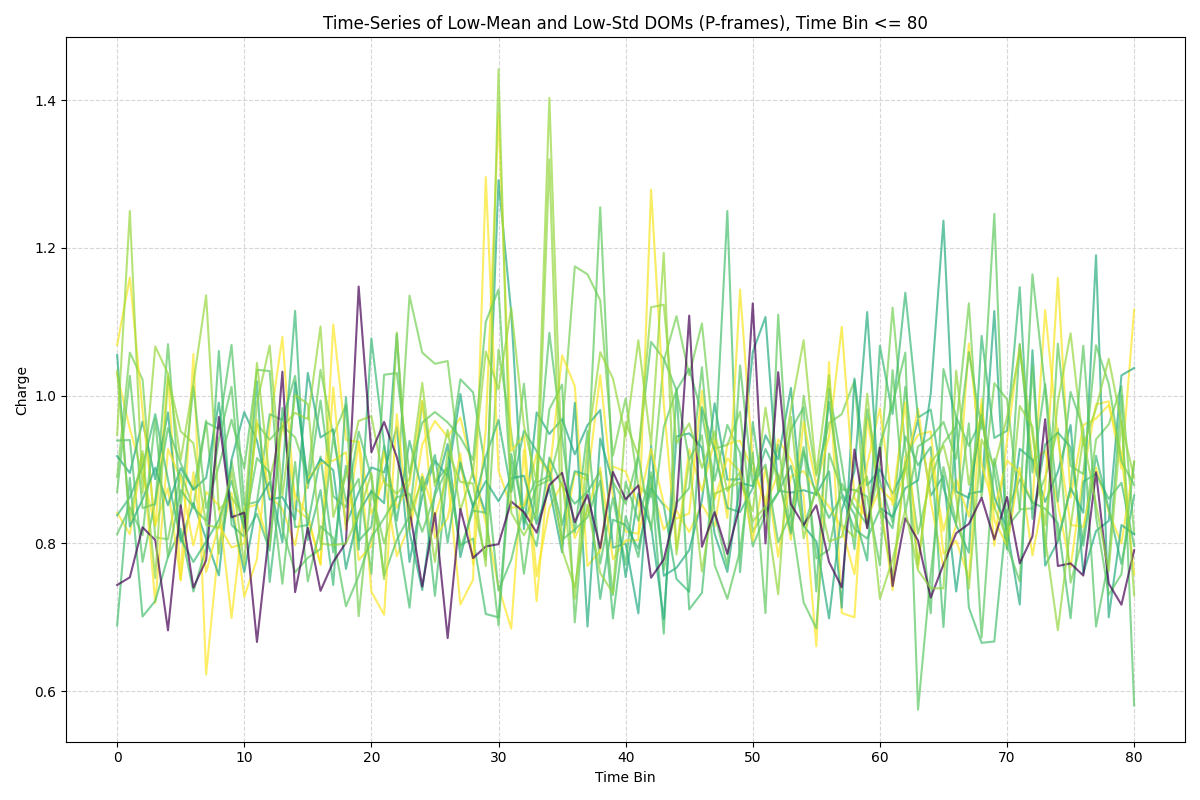
\includegraphics[width=0.7\textwidth]{Plots/q_high_mean_charges_t80.png}
    \caption{p low mean charges cut}
\end{figure}

As an idea to filter out coincident events, some conditions where set to look for clusters of signals within singular DOMs. Here is the plot created.

\begin{figure}
    \centering
    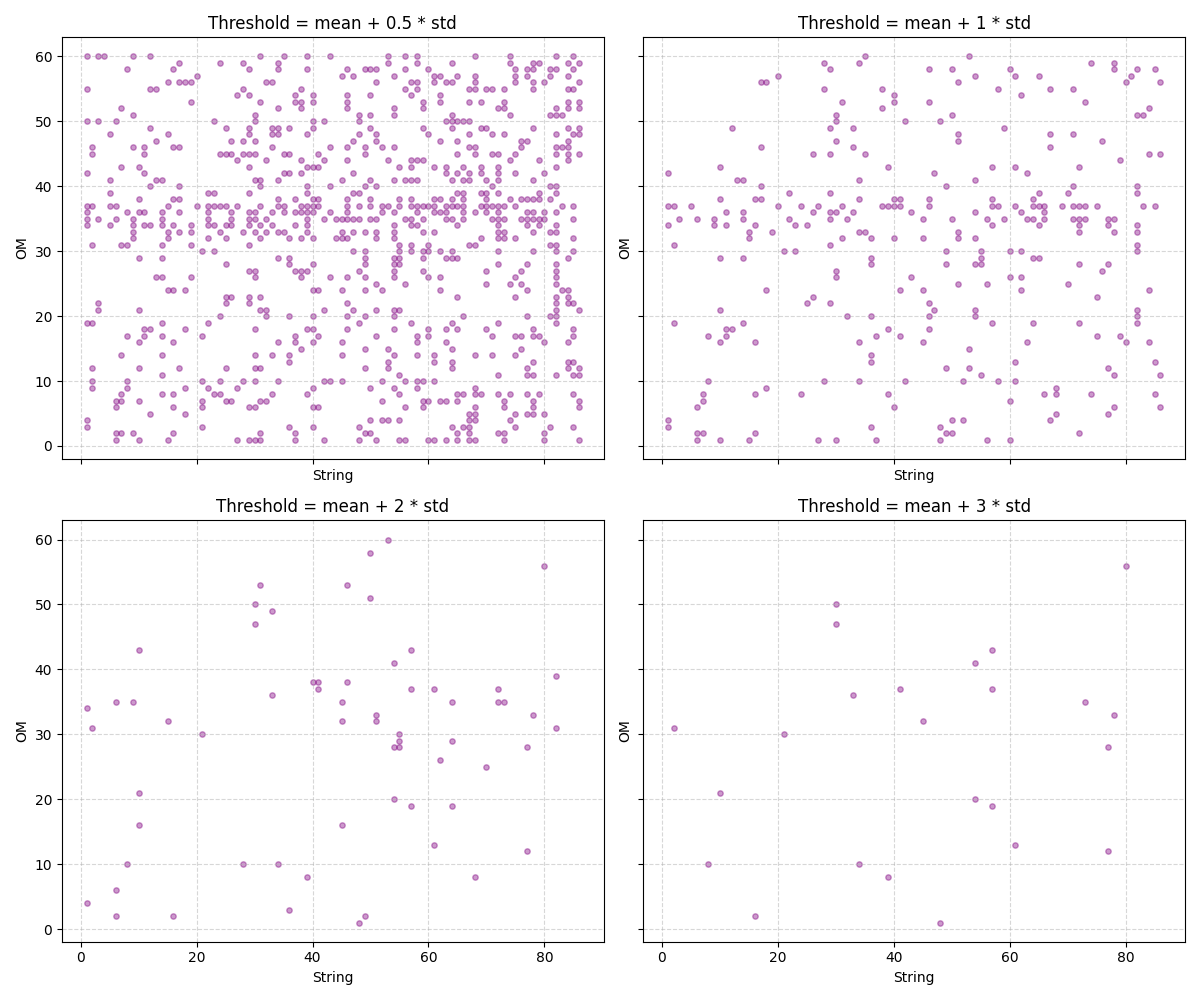
\includegraphics[width=0.7\textwidth]{Plots/p_high_mean_counts.png}
    \caption{p high mean counts}
\end{figure}
% \section{Description of plots for later use}
% \begin{figure}
%     \centering
%     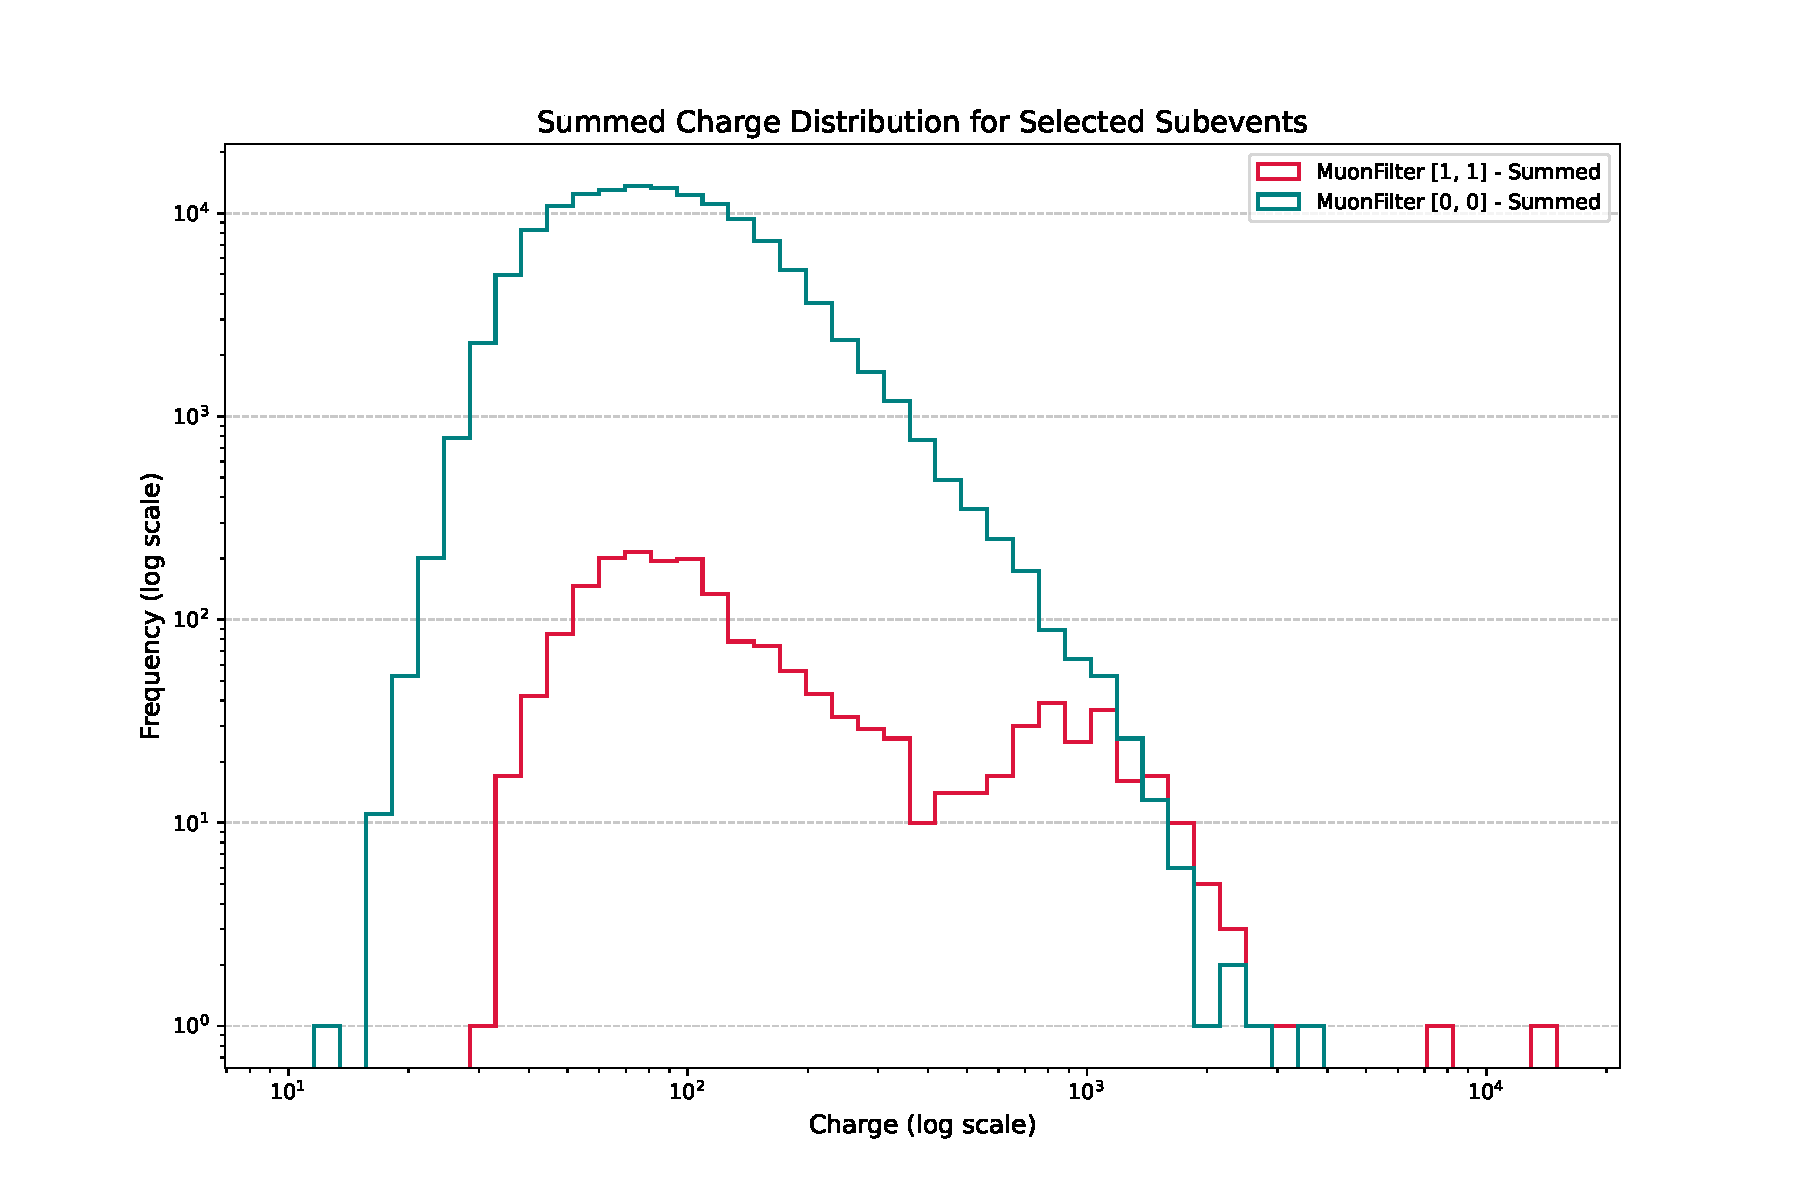
\includegraphics[width=0.7\textwidth]{Plots/frt_muon_filter_sub.pdf}
%     \caption{histogram showing FRT-subevents which did and did not pass the muon filter.}
%     \label{fig:frt_mu_sub}
% \end{figure}

% \begin{figure}[H] % The [H] forces the figure to be placed exactly here
%     \centering
%     \begin{subfigure}{0.49\textwidth}
%         \centering
%         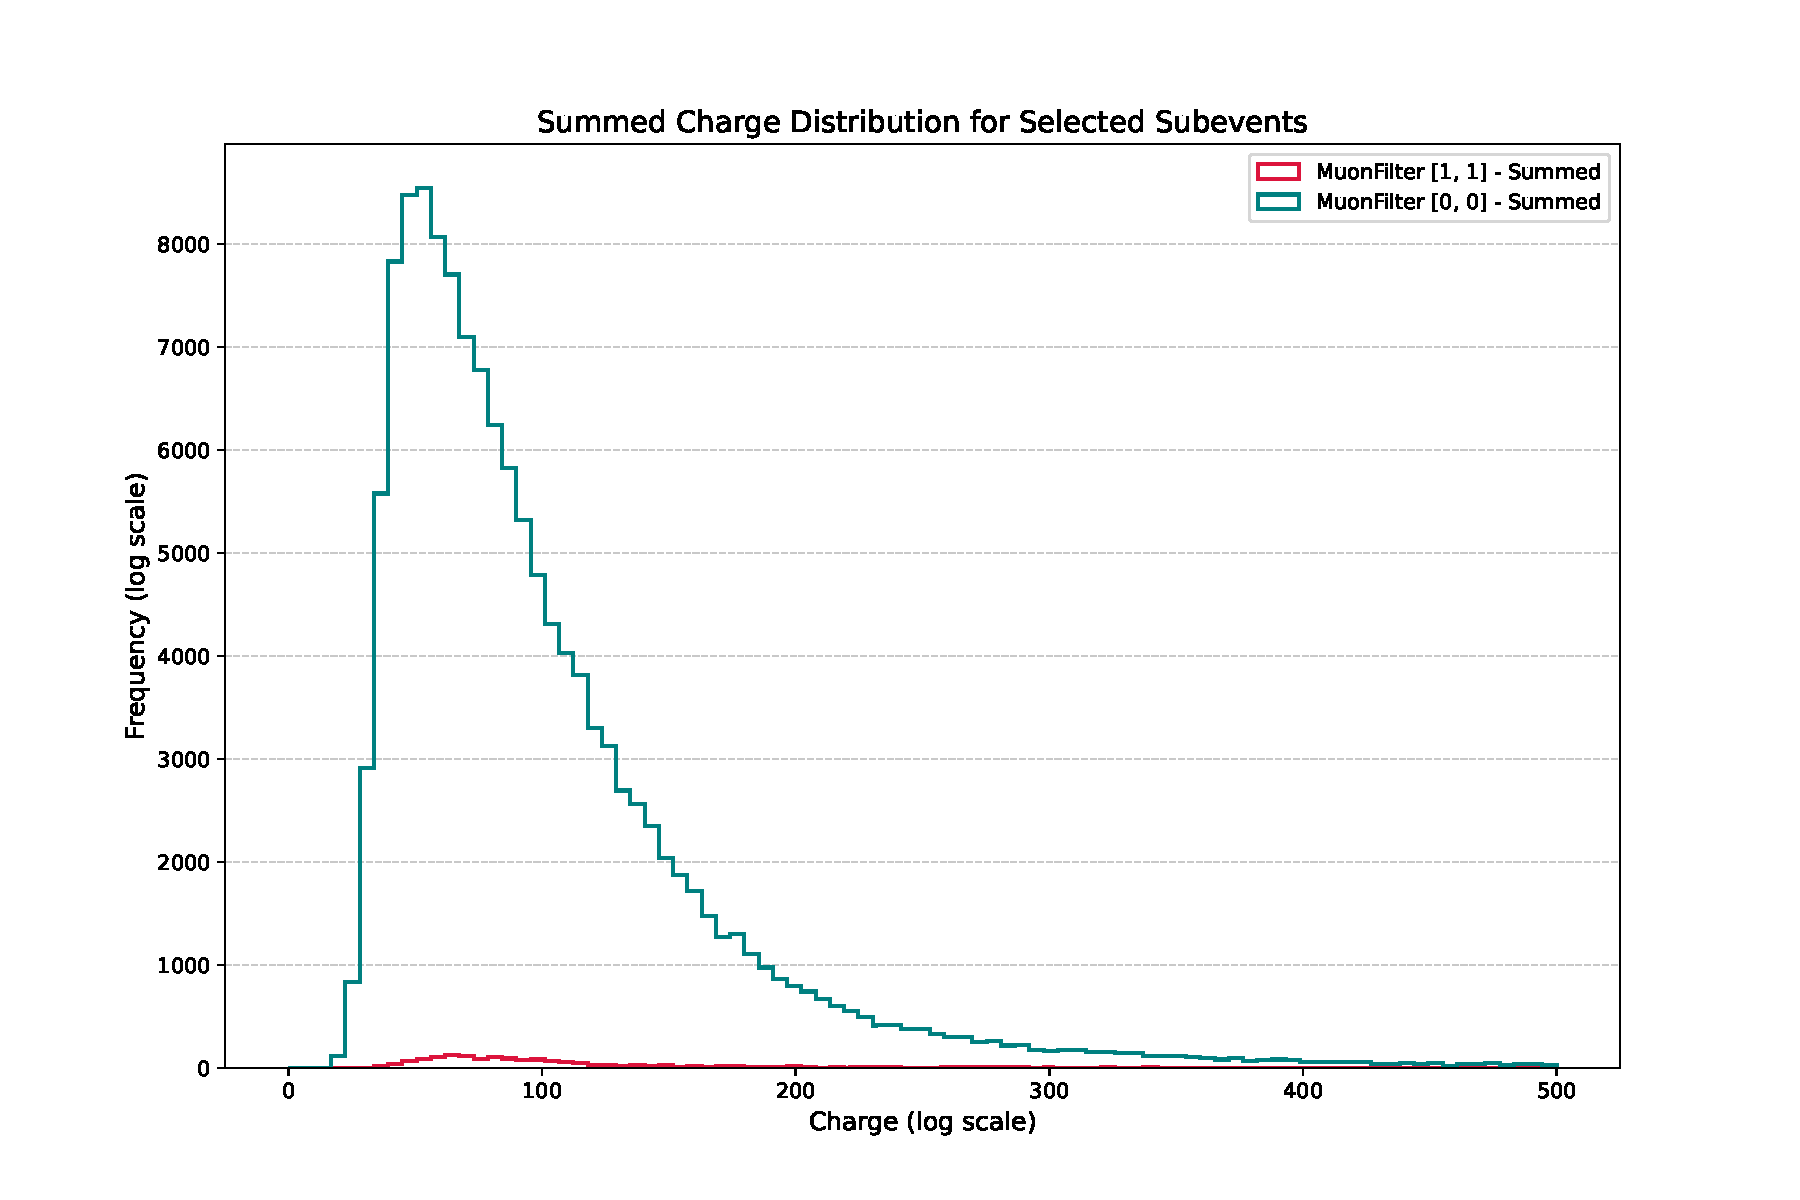
\includegraphics[width=\textwidth]{Plots/frt_muon_filter_sub_lin.pdf}
%         \caption{Subfigure 1}
%         \label{fig:sub1}
%     \end{subfigure}
%     \hfill % Adds spacing between the subfigures
%     \begin{subfigure}{0.49\textwidth}
%         \centering
%         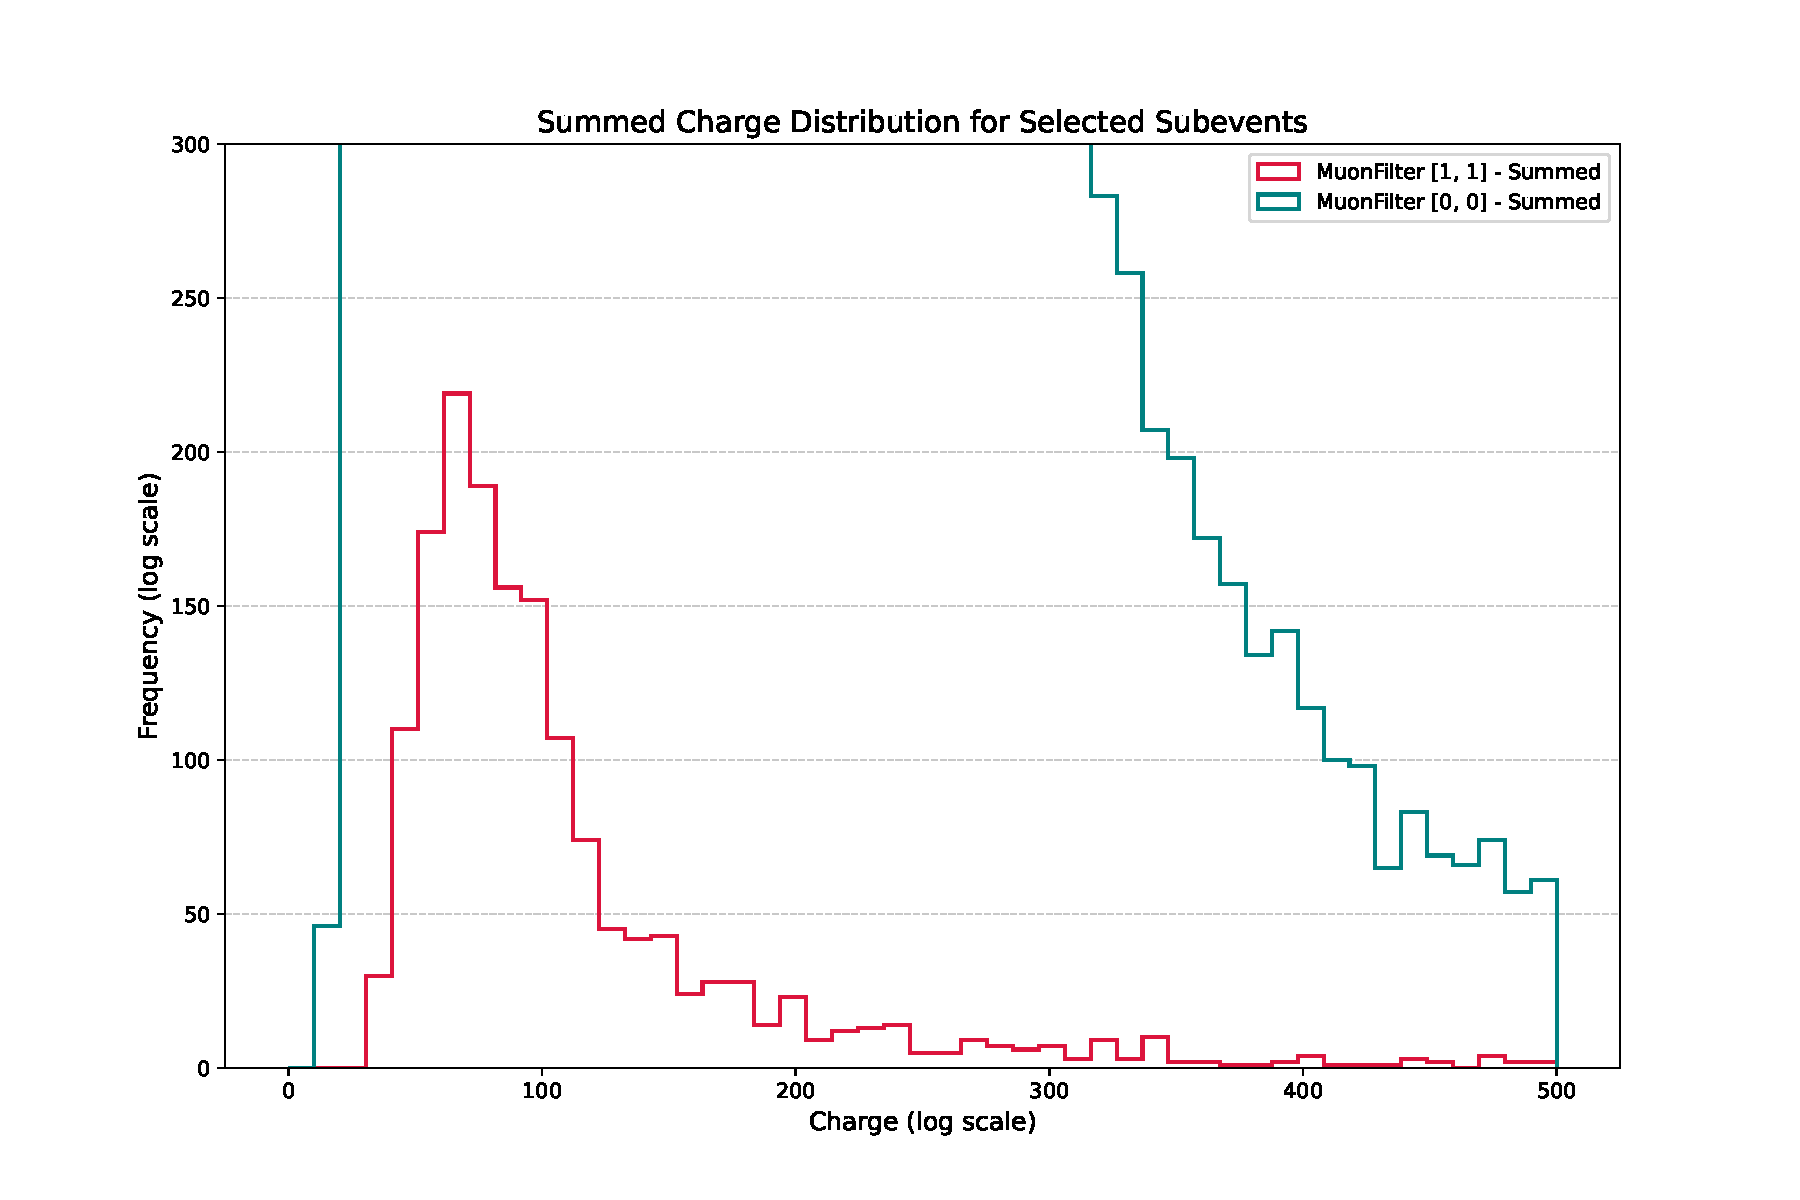
\includegraphics[width=\textwidth]{Plots/frt_muon_filter_sub_mod1.pdf}
%         \caption{Subfigure 2}
%         \label{fig:sub2}
%     \end{subfigure}
%     \caption{Main caption describing both plots.}
%     \label{fig:frt_mu_sub_comp}
% \end{figure}

% Figure~\ref{fig:frt_mu_2} shows the spectrum of \num{5032} FRT events, aswell as the spectrum of a subset of those events, which passed the muon filter, categorizing 
% them as muon events. The expectation here is that the muons event would have a charge distribution shifted to the right of the distribution making up the events 
% that do not satisfy the muon filter. This is assuming that whatever does not pass the muon filter is mostly noise. Any kind of background is expected to consist
% of signals carrying significantly less energy than the muons hitting the detector. Evendetly, this expectation is not fully satisfied by the histogram in 
% figure~\ref{fig:frt_mu_2}. While at higher charge values, the muon events start to make up the majority of the counts, the counts in these regions do not make up 
% a significant portion of the muon events themselves. Also, the peak of the muon events spectrum lies at around \num{2000}~PE, almost the same as the peak of the 
% failed events. The majority of both event types lie within the same region of charge values, meaning that there is a significant overlap in their distribution, 
% which makes a discrimination of muon event based solely on the charge measured by the detector, not directly possible. 
% \begin{figure}
%     \centering
%     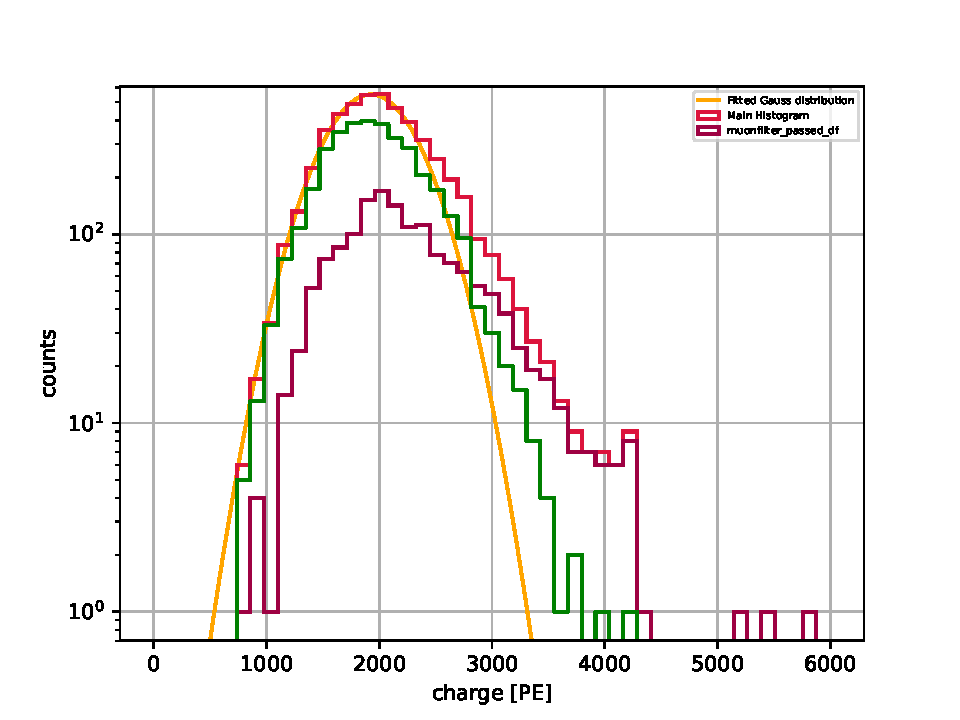
\includegraphics[width=0.7\textwidth]{Plots/frt_muon_filter.pdf}
%     \caption{histogram showing FRT-events which did and did not pass the muon filter.}
%     \label{fig:frt_mu_2}
% \end{figure}

% Another analysis can be made comparing the the q frames and p frames of the events collected by the FRT, as explained in section~\ref{sec:daq}. A comparison can be seen in 
% figure~(). Very similarly to the comparison of the events that pass the muon filter with those that fail, no significant difference can be seen in the two distributions. 
% It seems that something entirely disconnected from the charge left in the detector determines the distinction between physical events and noise. Even if this is true, 
% the two distributions appear almost identical in shape, which leads to the assumption that something might have went wrong in the processing of the data. 

% \section{coincidence probability}

% Assuming the capability to detect coincident events by their signature in the DOMs, the question still arises, what exactly constitutes the coinciding event. As 
% there seems to be a significant probability for an event leaving a signature similar to that of a muon, but not being one. In the following segment, an estimation
% can be made on how likely it is for a coincident event to be a true coincident muon, based on different types of knowledge about the event. 


